% This is samplepaper.tex, a sample chapter demonstrating the
% LLNCS macro package for Springer Computer Science proceedings;
% Version 2.21 of 2022/01/12
%
\documentclass[runningheads]{llncs}
%
\usepackage[T1]{fontenc}
% T1 fonts will be used to generate the final print and online PDFs,
% so please use T1 fonts in your manuscript whenever possible.
% Other font encondings may result in incorrect characters.
%
\usepackage{amsmath}
\usepackage{graphicx}
\usepackage{amssymb}
\usepackage{algorithm}
\usepackage{algpseudocode}
\usepackage{tikz}
\usepackage{fixme}
\usepackage{url}
\usepackage{booktabs}
\usetikzlibrary{arrows.meta, positioning}
\fxsetup{status=draft} % <====== add this line
 
\usepackage{graphicx}
\usepackage{subcaption}

% Used for displaying a sample figure. If possible, figure files should
% be included in EPS format.
%
% If you use the hyperref package, please uncomment the following two lines
% to display URLs in blue roman font according to Springer's eBook style:
%\usepackage{color}
%\renewcommand\UrlFont{\color{blue}\rmfamily}
%\urlstyle{rm}
%
\begin{document}
	
	\title{On Solving the Multiple Variable Gapped Longest Common Subsequence Problem}
	%
	\titlerunning{On Solving the MVGLCSP}
	
	\author{
		Marko Djukanović\inst{1,2, 6}  \and
		Nikola Balaban\inst{1}   \and
		Christian Blum\inst{3}  \and 
		Aleksandar Kartelj\inst{4}  \and
		Sašo Džeroski\inst{5}  \and
		Žiga Zebec\inst{6}
	}
	%
	\authorrunning{Djukanovic et al.}
	
	\institute{		University of Nova Gorica, Nova Gorica, Slovenia \\ \email{marko.dukanovic@ung.si} \\ \and Faculty of Natural Sciences and Mathematics, University of Banja Luka, Banja Luka, Bosnia and Herzegovina \\
		\email{nikola.balaban@student.pmf.unibl.org}, \email{marko.djukanovic@pmf.unibl.org} \and
		Artificial Intelligence Research Institute (IIIA-CSIC), Barcelona, Spain \\
		\email{christian.blum@iia.csic.es} \and 
		Faculty of Mathematics, University of Belgrade, Belgrade, Serbia \\ \email{kartelj@matf.rs} \\ \and
		Jožef Stefan Institute, Ljubljana, Slovenia \ \\ \email{saso.dzeroski@ijs.si}  \\
		\and
		Institute of Information Sciences (IZUM), Maribor, Slovenia \\
		\email{ziga.zebec@izum.si}
	}
	%
	\maketitle              % typeset the header of the contribution
	%
	\begin{abstract}
	     This paper tackles the variable gapped longest common subsequence problem, a variant of the well-known longest common subsequence (LCS) problem with an arbitrary large set of input strings. The problem has an application in comparing molecular sequences allowing structural distance constraints between nucleotides,  and time series analysis where the events occur within specified temporal delays. The proposed methodology first employs   root-based state graph definition, and the definition of the full state space given as the union of, in general, a large number of root-based state graphs. To deal with this issue,  
	      an iterative beam search approach is employed by utilizing a global, dynamically generated set of root nodes to control the diversification of the approach.   To guide the search of standalone beam search, several heuristic guidances from the LCS literature are probed. For the first time, the computational experiments on this general problem are performed by generating {300} synthetic problem instances. Our iterative approach has shown the best performance when compared to the baseline beam search and \textcolor{red}{a greedy approach} employing comparable amount of time for the former two. Moreover, for the special case with two input strings, our iterative   strategy approach could obtain an optimal solution on more than 80\% of problem instances with two input strings,  solved by all three dynamic approaches from literature.  
	\keywords{Longest common subsequences  \and Beam Search  \and Bioinformatics \and Gap constraints}
	\end{abstract}
	%
	%
	%
    \section{Introduction}
	
	The \textrm{Longest Common Subsequence Problem} (LCSP)~\cite{DJUKANOVIC2020106499,bergroth2000survey} is a well-known combinatorial optimization problem with numerous applications in bioinformatics and computational biology, particularly useful in the analysis of molecular sequences. Given an arbitrary large set of input sequences  $S=\{s_1,\ldots,s_m\}, m\in \mathbb{N}$  over an alphabet $\Sigma$, we aim to identify the longest possible subsequence common to all $s_i \in S$. In recent decades, many practically motivated variants of the LCSP have been proposed by considering additional structural or biological constraints. Among the well-known  variants are the constrained, arc-preserving, repetition-free~\cite{jiang2004longest,farhana2015constrained,adi2010repetition}, etc.
	
	In this work, we focus on solving the \textit{Variable Gapped Longest Common Subsequence Problem} (VGLCSP), introduced in~\cite{penga2011longest} for two input strings, and also theoretically examined in~\cite{adamson2023longest}. This problem extends the standard LCSP by imposing flexible distance limits (``gaps'') between consecutive symbols in the resulting subsequence, allowing these gaps to vary along the input sequences. Formally, for each input sequence $s_i \in S$ and  gap function/constraint  $G_{i}\colon \{1,\ldots,|s_i|\}\mapsto \mathbb{N}$ if the characters of a subsequence $s$ appear at the positions $i^1_i < \ldots < i^{{|s|}}_i$ in $s_i$, we say that the gap constraint is satisfied if $i^x_i - i^{x-1}_i \le G_{s_i}[i^x_i] + 1$ for all $x=2,\ldots,|s|$. A common subsequence $s$ is considered feasible if the corresponding gap constraints hold across all sequences in $S$. The VGLCSP represents a flexible and realistic model of sequence alignment, which is particularly useful for comparing DNA or protein sequences with variable structural distances. Another application includes the time series analysis and specially the events that must occur within specified temporal delays~\cite{lainscsek2015delay}.
	
	Although several exact dynamic programming approaches exist for the two-sequence case ($m=2$)~\cite{penga2011longest}, their computational complexity becomes prohibitive for larger $m$. To the best of our knowledge, no effective exact or approximate approaches are currently existing for the generalized VGLCSP with arbitrary large set $S$, which is clearly an NP-hard problem as a general version of the LCS problem with arbitrary large set of input strings. 
	
	\subsection{Preliminaries and Notation}
	  
	  Before presenting the algorithmic concept of the tackled problem, the common notation used throughout this work is introduced.
	  
	  Let $|s|$ denote the length of a sequence $s$. The term $s[i]$ refers to the character at the $i$-th position of sequence $s$, where the first position is indexed by $i = 1$. The substring of $s$ that begins at index $i$ and ends at index $j$ is denoted by $s[i, j]$; if $i = j$, this corresponds to the single character $s[i]$, whereas if $j < i$ then $s[i, j] = \varepsilon$, where $\varepsilon$ denotes the empty string.
	  
	  The number of occurrences of a character $a \in \Sigma$ in a sequence $s$ is denoted by $|s|_a$. For a subset of characters $\Sigma' \subseteq \Sigma$, the number of occurrences of characters from $\Sigma'$ in $s$ is defined by
	  \[
	  |s|_{\Sigma'} = \sum_{\sigma \in \Sigma'} |s|_{\sigma}.
	  \]
	  
	   We use $S = \{s_1, \ldots, s_m\}$ to denote the set of input sequences, and unless stated otherwise, $n$ denotes the length of the longest sequence in $S$, and $m\in \mathbb{N}$ the number of input sequences (corresp. gaps constraints). \\
	  %DEFINITION OF VGLCS PROLEM: TODO
	  
	The remainder of the paper is organized as follows. Section~\ref{sec: state_graph} explains the state graph of the tackled problem. In Section~\ref{sec: imsbs} we provided a design of our main methodological contributions through the iterative multi-source beam search approach. Section~\ref{sec: experiments} reports the empirical evaluation between our approach, the baseline standalone beam search and a greedy approach along with the special case of the instances with two input sequences. Finally, Section~\ref{sec: conclusions} provides conclusions and an outline for future work. 
	
	\section{Root-based State Space Formulation}\label{sec: state_graph}
	
      Building on already established LCSP state-space representation from~\cite{DJUKANOVIC2020106499}, we design a root-based \textit{state graph} model for the VGLCSP. Each state represents (one or more) feasible partial solutions  defined by the vector of positions induced by each input sequence and the solution length. Symbolically, a partial subsequence $s^v$ induces the state node $
v = (\mathbf{p}^{L,v},\, l^v) $ if: (i) $p^{L,v}_i - 1$ represents the smallest index in $s_i$ such that $s^v$ is a subsequence of $s_i[1,s_i[p^{L,v}_i - 1]$; (ii) $l^v = |s^v|$, and (iii) all gap constraints $G_{s_i}$ in the case of $s^v$ are satisfied. 

A directed arc $\alpha = (v_1 v_2)$, labeled with $lett(\alpha) = a \in \Sigma$, exists if
$l^{v_2} = l^{v_1} + 1 \quad \textrm{and} \quad s^{v_2} = s^{v_1} \cdot a$, for a partial solution $s^{v_1}$ of $v_1$ and a partial solution $s^{v_2}$ of $v_2$. 

To expand a state $v$, only those letters $a \in \Sigma$ that appears in the suffix sequence of $s_i$ starting at position $p^{L,v}_i$, for each $i=1, \ldots, m$, are  considered. For each such letter $a$, minimal feasible positions $p^{L,a}_i \ge p^{L,v}_i$  so that $s_i[ p^{L,a}_i]=a$ are identified which fulfill
\[
p^{L,a}_i - p^{L,v}_i \le G_{s_i}(p^{L,a}_i), i=1, \ldots, m.
\]
A child node is then defined by
$w = (p^{L,a} + 1,\; l^v + 1)$, if not dominated by another child nodes.  
For the purpose of efficient calculation of child nodes and their positions, we make use of the following data structure, labelled \texttt{Succ}.  It is a 3-dimensional integer list of $(i, j, a)$, where $i$ refers to the sequences $s_i$, the $1 \leq j \leq |s_i|$ refers to the position inside the sequence $s_i$ and symbol 
$a\in \Sigma$. The $q=$\texttt{Succ}[$i, j, a$] represents the smallest index $q \leq j$ so that $s_i[q]=a$, and the gap constraint is satisfied at that position, i.e., $q-j \leq G_i(q) + 1$. If no such position, -1 is assigned. The stru


The root state is given by $r = ((1,\ldots,1), 0)$, representing the empty subsequence, while goal states correspond to non-expandable feasible states. The search space that starts with $r$ as the root node is denoted by ${Space}(r)$. The space clearly depends on the selected root node from where the search starts, as pointed in the next paragraph. 

% U nekom delu LaTeX dokumenta:
\begin{figure}[h!]
	\centering
	\scalebox{0.4}{
	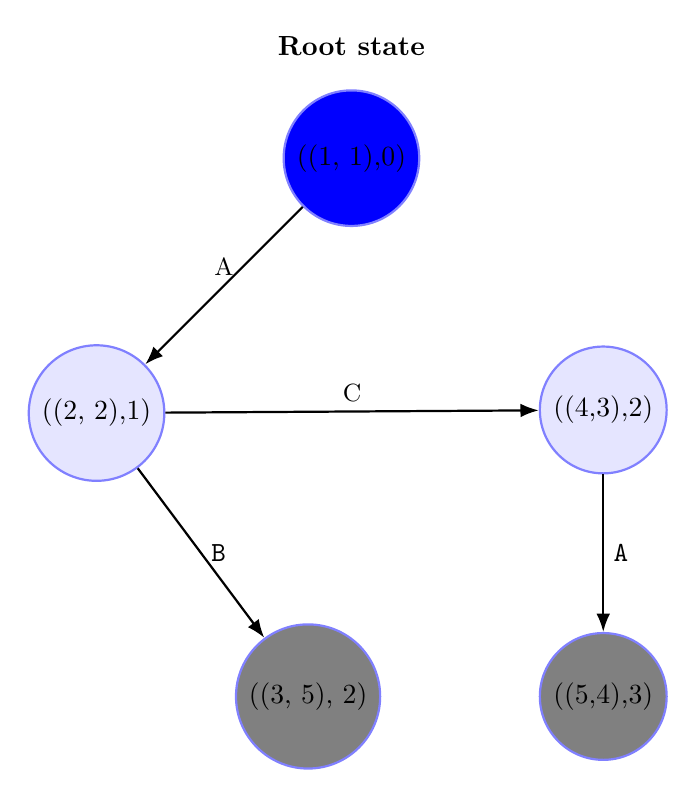
\begin{tikzpicture}[
		state/.style={circle, draw=blue!50, fill=blue!10, thick, minimum size=8mm},
		edge/.style={-Latex, thick},
		node distance=2cm and 2cm
		]
		
		% Čvorovi
		\node[state, fill=blue] (s0) {((1, 1),0)};
		\node[state, below left=of s0] (s1) {((2, 2),1)};
		\node[state, below right=of s0] (s2) {((4,3),2)};
		%\node[state, below=of s2] (s3) {(4,3)};
		\node[state, below=of s2, fill=gray] (s4) {((5,4),3)}; % krajnje, ali ne koristi se ovde
		\node[state, left=of s4, fill=gray] (s5) {((3, 5), 2)}; % krajnje, ali ne koristi se ovde
		
		% Grane (samo validne poklapanja)
		\draw[edge] (s0) -- node[above] {\small A} (s1);
		%\draw[edge] (s0) -- node[above] {\small A} (s2);
		\draw[edge] (s1) -- node[above] {\small C} (s2);
		%\draw[edge] (s2) -- node[right] {\small A} (s3);
		%\draw[edge] (s3) -- node[right] {\texttt{A}} (s4);
		\draw[edge] (s1) -- node[right] {\texttt{B}} (s5);
		% Oznake
		\node[above=0.3cm of s0] {\textbf{Root state}};
		%\node[below=1.5cm of s3] {\small \textbf{Krajnje stanje}};
		\draw[edge] (s2) -- node[right] {\texttt{A}} (s4);
		
	\end{tikzpicture}}
	\caption{State graph $Space(((1, 1), 0))$ for MVGLCSP between the sequences \texttt{ABCA} i \texttt{ACAB}. Two final/terminal states are displayed in gray. }
	\label{fig:vgcs-grafstanja}
\end{figure}

\paragraph{Motivation for Multi-Source Beam Search.} Unlike in the classical LCSP, the VGLCSP may contain multiple (potentially exponentially many) disconnected root components. For instance, in the sequences $S=\{
s_1 = \texttt{ATGGAAAA}, s_2 = \texttt{ATCCAAAA} \}$
with gap limits $G_{s_1} = G_{s_2} = 1$ presented in Fig.~\ref{fig:vgcs-grafstanja}, the initial state $((1,1),0)$ cannot reach any state node with the position vector $\mathbf{p}^L = (5,5)$. As a result, the optimal subsequence \texttt{AAA} becomes unreachable under traditional expansions and therefore missed out when starting at the root node $((1,1),0)$.  \\
 Following this, the full state space is defined as $\bigcup_{q \in \mathcal{R}} Space(q)$, where $\mathcal{R}$ represents a set of all root nodes/states $v$ with its positions $p^{L, v}$ which cannot be reached from any other state %, that is a state with  position vector $p^{L, w}$, $p^{L, w}_i < p^{L, v}_i$, for each $i=1, \ldots, m$, 
 through regular directed transitions. Unfortunately, enumerating all root nodes in the search space of an VGLCS problem instance is, in general, a time consuming task, executed in $O(n^m)$ time, thus is hardly doable when $m$ or $n$ is huge.  This structural property motivates our \textit{Iterative Multi-Source Beam Search} (IMSBS) approach, specifically designed to explore multiple promising start regions of the state space and overcome disconnection issues caused by the gap constraints,  inherent to the VGLCSP.

	
	\section{Iterative Multi-source Beam Search Framework}\label{sec: imsbs}
	
	\textit{Beam search} (BS) is a popular tree-search meta-heuristic approach which performs in a breadth-first-search manner, where the search is controlled by the parameter $\beta$  referring to as the number of nodes to be further expanded at the considered level, and a guiding function $h$ to make the decisions about  which nodes to select for further expansions. 
	
	In the \textit{Iterative Multi-source Beam Search}  (IMSBS) framework, BS is iteratively executed with an initial set/beam $\mathcal{L}$ of promising root nodes, which are popped from a dynamically maintained global pool $\mathcal{R}$ of root nodes. This set serves to control the diversification of the approach.  
   The single beam search utilized several heuristics to intensify the search towards producing feasible solutions; those  are based on letter frequencies, minimal residual substring lengths, or probability-weighted estimates as  provided in the next sections. \\
    
    Pseudocode of the approach is given in Algorithm~\ref{alg:imbs}. First, a pool of root nodes  $\mathcal{R}$ comprising of the root node $r=((1, \ldots, 1), 0)$ is initialized, referring to the empty partial solution $s_{\mathrm{best}}=\varepsilon$. The algorithm runs until $\mathcal{R}$ is empty or the number of BS calls is exceeded (provided as the algorithm's parameter). At each iteration, the following instructions are executed. First, several most promising root nodes (parameterized by  \emph{number\_of\_sources\_from\_R})  according to heuristic evaluation $h'$ have been selected from $\mathcal{R}$, subsequently  stored into a temporal beam $\mathcal{L}$, serving as the initial beam,  used in the current beam search procedure executed with a beam width $\beta$ and a heuristic guidance $h$. During the execution, all completed (non-expandable) nodes are  processed in the following way: If a new best solution has been found, $s_{\textrm{best}}$ is updated accordingly.  Each such complete node is then independently expanded in an LCS-manner (ignoring gaps), generating a set of children. For a generated child with position vector  $p^w$, if $|s_i| - p^w_i +1 \leq |s_{\mathrm{best}}|$ holds for at least one index $i\in [m]$, it is  omitted for further consideration  as a proven suboptimal transition; otherwise, $r^w=(p^w, 0)$ has been added to $\mathcal{R}$ as a candidate for root node  if not been already generated in the  previous iterations (i.e., no duplicate root nodes are or had already been in the pool). When the beam search has completed, a subsequent beam search  is started with a new set of (root) nodes taken from $\mathcal{R}$ if none of the conditions for termination is met. Note that the pool $\mathcal{R}$ is organized as a priority queue (binary heap). 
    
    
     
    
    %pseudocode:
    \begin{algorithm}[!ht]
    	\caption{Iterated Multi-source Beam Search (IMSBS) Framework }
    	\label{alg:imbs}
    	\begin{algorithmic}[1]
    		\Require Sequences $s_1, \dots, s_m$; Gap functions $G_{s_i}(\cdot)$; beam width $\beta>0$; ${number\_sources\_from\_R}>0$; $beam\_iters>0$, heuristics $h, h'$
    		\Ensure Approximate common subsequence $s_{\textrm{best}}$
    		
    		\State Initialize $\mathcal{R} \gets \{ (\mathbf{1},0) \}$ \Comment{A set of root nodes}
    		\State $iter \gets 0$
    		\State $s_{\textrm{best}} \gets  \varepsilon$
    		
    		\While{$\mathcal{R} \neq \emptyset \wedge iter < beam\_iters $ }
    		\State Select $\mathcal{L} \subseteq \mathcal{R}$  ${number\_sources\_from\_R}$ nodes, \State Remove the selected nodes from $\mathcal{R}$
    		\Comment{$\mathcal{R}$ can be a pr. queue ordered by heuristic $h'$}
    		\State Execute beam search $BS( \mathcal{L}, h)$
    		
    		\ForAll{complete nodes $v$ at $BS(\mathcal{L}, h)$}
    		\ForAll{Symbol $a \in \Sigma$}
    		\State $p^w \gets$ minimum positions in the sequences so that $\ge p^v$ and $s_i[p^w_i] = a$ (ignore all gap constraints)
    		\If{$|s_{\textrm{best}}| < \min_{i=1,\dots,m} \{ |s_i| - p^w_i + 1 \}$}    \Comment{cut-off}
    		\State Add $r^w = (p^w,0)$ in the set  $\mathcal{R}$ (if previously have not added)
    		\EndIf
    		\EndFor
    		\EndFor
    		
    		\State Update $s_{\textrm{best}}$ if a new longest subsequence  in $BS(\mathcal{L}, h)$ has been found
    		\State $iter \gets iter + 1$
    		\EndWhile
    		
    		\State \Return $s_{\textrm{best}}$
    	\end{algorithmic}
    \end{algorithm}
    The core advantages of the IMSBS approach over the baseline BS are: 
    \begin{itemize}
    	\item It provides a heuristic balance between beam search (local exploration of promising paths) and the generation of new sources (global coverage of the search space).
    	\item Filtering suboptimal root nodes reduces unnecessary iterations and enables pruning of dominated paths.
    \end{itemize}

    \subsection{Heuristic guidances}
    
    Several heuristics to guide search are utilized within the IMSBS (as the candidate for $h$ and $h'$). 
    \begin{itemize}
    	\item  \textit{``Look-ahead'' for the remaining length:}
    	\begin{equation}
    		\textrm{UB}_1(\mathbf{v}) = \min_{i = 1, \ldots, m} \left( |s_i| - p_i^v + 1 \right)
    	\end{equation}
    	This is an estimate of the potential extension of the sequence up to the end of the shortest remaining sequence.
    	
    	\item  \textit{Character Frequency Alignment:}
    \begin{equation}
    	\textrm{UB}_2(\mathbf{v}) =  \sum_{\sigma \in \Sigma} 
    	\min\left(  |s_1[p_1^v, |s_1|]|_{\sigma}, \ldots, |s_m[p_m^v, |s_m|]|_{\sigma} \right)
    \end{equation}
    In essence, this heuristic counts the maximum number of characters that can still match in the (optimal) solution based on the frequency of each character. This score can be computed efficiently in \(O(m)\) time using preprocessing (i.e., constructing suitable data structures), see~\cite{DJUKANOVIC2020106499}. 
     \item \textit{A probability-based heuristic} guidance by the Mousavi and Tabataba's matrices from~\cite{mousavi2012improved} in the context of the LCS problem. These probabilities are based on the idea of determining a probability for the event realization that a sequence $s$ of length $k$ is a subsequence of a (random) sequence of length $n$ over an alphabet $\Sigma$.  The probabilities for each  $i=1,\ldots, k$ and  $j=1, \ldots, n$, are pre-processed by a matrix $\mathcal{P}$ of probabilities of dimension $k\times n$ by a dynamic programming recurrence. Assuming the independence betwen input sequences, at each level of beam search the nodes are evaluated by determining the probabilities for each partial solutions  across that level to be expanded by $\overline{k}$ letters (this value is heuristically evaluated, as proposed in~\cite{mousavi2012improved}). Denote that heuristic guidance   by $h_{\textrm{prob}}$. 
     \item TODO: \fxnote{TODO: if we come up with some learning heuristic -- should left for the extended version -- journal-extendable.}
   \end{itemize}
    
	
\section{Experimental Evaluation}\label{sec: experiments}
   
In this section, we compare the results of heuristic approaches designed for the VGLCSP with arbitrary $m \geq 2$, namely:
\begin{itemize}
	\item The baseline beam search approach, that starts with the root node $r$ as the initial beam and runs a single iteration of IMSBS. We denoted it by \textsc{Bs}. 
	
	\item The tuned iterative multi-source beam search, given in Algorithm~\ref{alg:imbs}, denoted by \textsc{Imsbs}, that uses comparable runtime to those of the \textsc{Bs}.
	\item  The IMSBS for the fixed $\beta=1$, given in Algorithm~\ref{alg:imbs}, denoted by \textsc{Imsbs-greedy}, that show the influence of larger number of BS iterations on the performance of the \textsc{Imsbs}. 
\end{itemize}

The \textsc{Imsbs} is implemented in Python 3.11, and evaluated on the HPC VEGA Supercomputer placed at IZUM, Maribor. This is a cluster of has 960 nodes, 1920 CPUs with AMD Epyc 7H12, and 2.35GHz.  All experiments were executed in a single-threaded setting.
   
   
   \subsection{Instance generation}
    
  For each combination of instance parameters $n \in \{50, 100, 200, 500\}$, $m \in \{2, 3, 5, 10\}$, and $|\Sigma| \in \{2, 4\}$, 
  10 random problem instances are generated.  First, $m$  equally-size sequences  generated uniform-at-random. Then, the gap constraints for each instance (i.e., positions of sequences) are generated so that for each $G_i(j), j=1, \ldots, |s_i|, i=1, \ldots, m$, assigned is a value 
  $G_{s_i}(j) \in \mathcal{U}(\{ \lfloor 0.5 \cdot |\Sigma| \rfloor, \ldots, \lfloor 1.5 \cdot |\Sigma| \rfloor \})$.   Therefore, a total of 320 problem instances are generated; the benchmark set is denoted as \textsc{Random}. All instances from the \textsc{Random} dataset can be found at   
  \url{https://github.com/markodjukanovic90/NikolaBalabanDiplomski/tree/main/src/instance_i_generator}.
 \subsection{Parameter tuning}
      For the \textsc{Bs} approach, a high beam width $\beta = 10,000$ and $h=\mathrm{h}_{prob}$ is utilized as no significant increase in the solution quality of the \textsc{Bs} by further increasing the the size of beam, while ${h}_{prob}$ provided a slightly better guidance from $\textrm{UB}_2$ but significantly better from $\textrm{UB}_1$; see Fig.~       	\ref{fig:bs_tuning}.
      
\begin{figure}[!ht]
	\centering
	\begin{subfigure}[t]{0.48\textwidth}
		\centering
		\includegraphics[width=\linewidth, height=120pt]{figures/bs_tuning_quality.png}
		\caption{Avg. quality over all benchmark suite \textsc{Random}.}
		\label{fig:tune_bs}
	\end{subfigure}
	~
	\begin{subfigure}[t]{0.48\textwidth}
		\centering
		\includegraphics[width=\linewidth, height=120pt]{figures/bs_tuning_time.png}
		\caption{Avg. runtime over all benchmark suite \textsc{Random}.}
		\label{fig:tune_bs_time}
	\end{subfigure}
	\caption{Beam search tuning results on the \textsc{Random} benchmark suite.}
	\label{fig:bs_tuning}
\end{figure}
 
      
      After conducting a series of preliminary experiments, we agreed to fix the parameter   ${number\_sources\_from\_R} = 10$ and \emph{beam\_iters} is set to 50, as high-quality results have been already achieved with this amount of iterations. With the same reason, root nodes that are kept in the global set of root nodes are prioritized according to  $h'=\textrm{UB}_2$, which allowed the IMSBS to performed consistently better when the $\textrm{UB}_1$.    The remaining parameters of IMSBS approach were tuned utilizing the simple grid search strategy with the following values $h \in \{ \textrm{UB}_1, \textrm{UB}_2, {h}_{prob}\}$ and $\beta \in \{ 100, 500, 2000\}$, see Fig.~\ref{fig:imsbs_tuning}. 
      
       
   \begin{figure}[!h]
   	\centering
   	\begin{minipage}{0.48\textwidth}
   		\centering
   		\includegraphics[width=\linewidth]{figures/imsbs_tuning.png}
   		\caption*{(a) Avg. quality for different settings of IMSBS over all instances from the benchmark suite \textsc{Random}.}
   		\label{fig:tune_imsbs}
   	\end{minipage}
   	~
   	\begin{minipage}{0.48\textwidth}
   		\centering
   		\includegraphics[width=\linewidth]{figures/imsbs_tuning_time.png}
   		\caption*{(b) Avg. runtime for different settings of IMSBS over all instances from the benchmark suite \textsc{Random}.}
   		\label{fig:tune_imsbs_time}
   	\end{minipage}
   	\caption{IMSBS parameter tuning runtime comparison on the \textsc{Random} benchmark suite.}
   	\label{fig:imsbs_tuning}
   \end{figure}
   
          
   In order to ensure a comparable average runtime consumption of IMSBS and the baseline \textsc{Bs} approach, we decided to use the following configuration for the IMSBS in our experimental evaluations:  $h=\mathrm{UB}_2$ and $\beta=500$. As already said, these values were chosen to strike a balance between allowed time resources relative to the baseline BS execution times while keeping reasonable final solution quality of \textsc{Imsbs}.  Similarly, due to the same reason, the \textsc{Imsbs-greedy} approach which has a fixed $\beta=1$, we allowed a budget of  {5000}  beam search iterations ($\emph{beam\_iters}=5000$), while other parameters were fixed to those values as in the case of the \textsc{Imsbs}. 
     
  
  \subsection{Numerical results for heuristic approaches }
   Numerical results for all three heuristic approaches are reported in  Table~\ref{tab:numerical_results_general_m},  organized into two main parts.
    The first three columns describe the instance characteristics, namely the number of sequences ($m$),
    the sequence length ($n$), and the alphabet size ($|\Sigma|$).
    The remaining columns report the performance of three heuristic approaches:
    \textsc{Bs}, \textsc{Imsbs-Greedy}, and \textsc{Imsbs}.
    For each algorithm, two performance indicators are provided:
    the average objective value $\overline{obj}$ and the average running time in seconds $\overline{t}[s]$ provided over 10 instances pera each group. 
    This organization allows a direct comparison of solution quality and computational effort across
    algorithms for identical instance settings.
     
    
    
    \begin{table}[H]
    	\caption{Numerical results of the three heuristic approaches on the \textsc{Random} benchmark suite. }\label{tab:numerical_results_general_m}
    	\centering
    	\scalebox{0.8}{
    	\begin{tabular}{lll|rr|rr|rr}
    		\hline
    		\multicolumn{3}{c}{Inst.} & \multicolumn{2}{c}{\textsc{Bs}} & \multicolumn{2}{c}{\textsc{Imsbs-Greedy}} & \multicolumn{2}{c}{\textsc{Imsbs}} \\
    		\cmidrule(lrr){1-3} \cmidrule(lr){4-5} \cmidrule(lr){6-7} \cmidrule(lr){8-9} \\ 
    		$m$ & $n$ & $|\Sigma|$ & $\overline{obj}$ & $\overline{t}[s]$ & $\overline{obj}$ & $\overline{t}[s]$ & $\overline{obj}$ & $\overline{t}[s]$ \\
    		\hline
\midrule
   2 & 50 & 2 & 33.6 & 0.02 & 26.1 & 0.00 & \textbf{35.0} & 0.04 \\
   2 & 50 & 4 & 30.1 & 0.89 & 24.8 & 0.00 & \textbf{30.1} & 0.14 \\
   2 & 100 & 2 & 48.9 & 1.74 & 41.5 & 0.00 & \textbf{65.1} & 0.44 \\
   2 & 100 & 4 & \textbf{62.1} & 9.75 & 50.5 & 0.00 & 61.6 & 0.67 \\
   2 & 200 & 2 & 99.1 & 14.76 & 67.7 & 0.01 & \textbf{123.3} & 3.20 \\
   2 & 200 & 4 & 120.5 & 38.56 & 74.8 & 0.01 & \textbf{120.9} & 3.55 \\
   2 & 500 & 2 & 65.3 & 21.05 & 77.3 & 0.03 & \textbf{184.9} & 62.69 \\
   2 & 500 & 4 & 214.6 & 155.30 & 152.4 & 0.02 & \textbf{222.8} & 35.27 \\ \hline
   
   3 & 50 & 2 & 17.5 & 0.02 & 17.4 & 0.00 & \textbf{25.8} & 0.05 \\
   3 & 50 & 4 & \textbf{21.7} & 0.17 & 16.1 & 0.00 & \textbf{21.7} & 0.09 \\
   3 & 100 & 2 & 19.7 & 0.07 & 25.2 & 0.00 & \textbf{46.6} & 1.42 \\
   3 & 100 & 4 & 34.1 & 2.50 & 21.1 & 0.00 & \textbf{42.3} & 2.49 \\
   3 & 200 & 2 & 15.2 & 0.15 & 29.2 & 0.01 & \textbf{73.6} & 9.63 \\
   3 & 200 & 4 & 85.3 & 24.99 & 38.3 & 0.01 & \textbf{91.3} & 33.44 \\
   3 & 500 & 2 & 12.6 & 0.10 & 36.0 & 0.04 & \textbf{57.0} & 21.62 \\
   3 & 500 & 4 & 90.7 & 80.60 & 52.6 & 0.03 & \textbf{149.2} & 171.48 \\ \hline
   
   5 & 50 & 2 & 4.8 & 0.00 & 9.4 & 0.00 & \textbf{15.3} & 0.06 \\
   5 & 50 & 4 & 8.9 & 0.01 & 7.1 & 0.00 & \textbf{12.2} & 0.11 \\
   5 & 100 & 2 & 6.3 & 0.00 & 10.3 & 0.01 & \textbf{16.2} & 0.16 \\
   5 & 100 & 4 & 5.3 & 0.01 & 7.4 & 0.01 & \textbf{18.7} & 0.41 \\
   5 & 200 & 2 & 5.3 & 0.01 & 14.5 & 0.01 & \textbf{19.2} & 0.31 \\
   5 & 200 & 4 & 6.4 & 0.02 & 10.6 & 0.02 & \textbf{22.6} & 0.68 \\
   5 & 500 & 2 & 5.9 & 0.09 & 15.2 & 0.08 & \textbf{21.5} & 1.32 \\
   5 & 500 & 4 & 6.8 & 0.10 & 13.4 & 0.08 & \textbf{20.5} & 1.15 \\ \hline
   
10 & 50 & 2 & 1.7 & 0.00 & 3.7 & 0.00 & \textbf{5.9} & 0.12 \\
10 & 50 & 4 & 1.9 & 0.00 & 2.7 & 0.00 & \textbf{4.4} & 0.31 \\
10 & 100 & 2 & 1.1 & 0.00 & 4.6 & 0.01 & \textbf{5.2} & 0.22 \\
10 & 100 & 4 & 2.2 & 0.01 & 2.8 & 0.01 & \textbf{4.1} & 0.47 \\
10 & 200 & 2 & 2.5 & 0.01 & 5.2 & 0.04 & \textbf{6.7} & 0.28 \\
10 & 200 & 4 & 2.2 & 0.01 & 3.7 & 0.04 & \textbf{3.9} & 0.43 \\
10 & 500 & 2 & 1.8 & 0.08 & 5.9 & 0.22 & \textbf{6.3} & 1.00 \\
10 & 500 & 4 & 1.9 & 0.08 & 4.2 & 0.23 & \textbf{4.6} & 1.27 \\  
	\hline \hline
\textbf{Avg.} &  &  &  32.38 & 10.97 & 27.24 & 0.03 &  \textbf{48.08} & 11.08  \\ \hline \hline
 \end{tabular}}
    \end{table}
    
 
    
    %beam_width-500_heuristic-h5_imbs-iters-50_num-roots-10: check here what is wrong ... 
 
    Based on the numerical results presented in Table~\ref{tab:numerical_results_general_m}, the following conclusions are drawn.  
    
    
    \begin{itemize}
    	\item \textit{Solution quality comparison.} \textsc{Imsbs} approach produces the highest solution quality in 31 out of 32 instance groups, on average exceeding the baseline \textsc{Bs} approach  by achieving a relative percentage  improvement of about 50\%.  The baseline BS approach performs  equally well or better in just 2 group.  The weakest (but also th fastest) in average performing approach is the \textsc{Imsbs-Greedy} approach. It performs fairly (and clearly better from \textsc{Bs}) only for the cases with a larger number of input sequences $m \in \{10\}$ which indicates on how wrong can be a decision of starting the beam search  from the root node $((1, 1), 0)$ due to many more gap constraints ($m$) to be fulfilled  and that exploring other root nodes quite often can be beneficial in improving diversity of the search, this affecting the quality of final solutions. 
    	  
    	 
    	\item \textit{Runtime comparison.}  The \textsc{Bs} and the \textsc{Imsbs} approaches have comparable average runtimes. As expected, a significantly smaller average runtime is exhibited for the \textsc{Imsbs-Greedy} approach mainly due to inexpensive beam search iterations utilized ($\beta=1$) in contrast to high-consuming beam search iterations in the other two approaches. 
     
    	 \item \textit{Other conclusions}. The behavior of \textsc{Bs} is explained by the fact that for small $m$, the choice of taking the root node $r = (1, \ldots, 1)$ is typically favorable, enabling BS to progress deeply and identify high-quality subsequences for higher beam widths. This is in particular the case of instances with $m=2$ where the difference between solution quality produced by \textsc{Bs} and \textsc{Imsbs} are in favor of the latter approach, but not that dramatically. When comes to larger values of $m$, one may notice huge gap between the solutions of these two.  Overall, IMSBS demonstrates considerably greater robustness and stability with respect to increased  number of input sequences.
    	
      %As illustrated in Figure~XX, both BS and IMSBS frequently attain near-optimal or optimal solutions for smaller $n$ and larger alphabets. The BS approach reaches at least 65\% of optimum for the majority of instances, whereas IMSBS achieves 80\% or more. For approximately 50 out of the 60 instances, both methods achieve at least 90\% of the optimal solution length, as shown in Figure~XX.
    \end{itemize}
    
    \subsection{Numerical results for the special case $m=2$}
     In this section, we compare the results of the literature approaches  specialized for the fixed $m=2$ case; the competitors are listed bellow and all are explained in detains in~\cite{penga2011longest}.
     
     \begin{itemize}
     	\item The basic dynamic programming algorithm, denoted as \textsc{Dp};
     	\item Advanced dynamic programming approach, that uses an Incremental
     	Suffix Maximum Queries (ISMQ) by utilizing \texttt{Col} and \texttt{All} matrices, to speed up the former approach, denoted as \textsc{Dp}-1;
     	\item Advanced dynamic programming algorithm which  Handling ISMQ by \textit{dequeue} data structure for further speeding up, denoted as \textsc{Dp}-2; all three DP approaches are from~\cite{penga2011longest}. Note that in the original paper, answering ISMQ with Union-find Operations is proposed. However, due to lack implementation details, we decided   to make use of the dequeue data structure in our implementation.
     	\item The integer linear programming method, denoted as \textsc{Ilp}, is proposed in this work, see Appendix~\ref{app:ilp}. It is motivated by the ILP model in the context of LCS problems~\cite{blum2016metaheuristics}. 
     \end{itemize}
     
     Each algorithm was given half an hour (30 minutes) of execution time. The \textsc{Ilp} model was solved using \textcolor{red}{the general-purpose solver \textsc{Cplex} version 22.1.}
     
     The results are provided in Table~\ref{tab:results-2d-literature}, which is organized as follows.
     The first three columns describe  characteristics of the instance groups over which the results are averaged (10 instances in each group). The next four blocks report the results of the four algorithms: \textsc{Dp}, \textsc{Dp}-1, \textsc{Dp}-2, and \textsc{Ilp}, respectively. For each approach, the   average solution quality and the average execution time is reported across 10 problem instances. 
     
     \begin{table}[H]
     	\caption{Results on the \textsc{Random} benchmark set for $m=2$: the exact approaches from the literature.}\label{tab:results-2d-literature}
     	\centering
     	\scalebox{0.7}{
     	\begin{tabular}{lll|lr|rr|rr|rr}
     		\hline
     		\multicolumn{3}{c}{Inst.} & \multicolumn{2}{c}{\textsc{Dp}}  &
     		\multicolumn{2}{c}{\textsc{Dp-1}} & \multicolumn{2}{c}{\textsc{Dp-2}} & 
     		\multicolumn{2}{c}{\textsc{Ilp}}  \\
     		\cmidrule(lrr){1-3} \cmidrule(lr){4-5}
     		\cmidrule(lr){6-7} \cmidrule(lr){8-9}
     		\cmidrule(lr){10-11} 	\\ 
     		$m$ & $n$ & $|\Sigma|$ & $\overline{obj}$ & $\overline{t}[s]$ & $\overline{obj}$  & $\overline{t}[s]$ &$\overline{obj}$  & $\overline{t}[s]$ & $\overline{obj}$  & $\overline{t}[s]$ \\
     		\hline
   2 &   50 &         2 &              38.1 &          0.01 & 38.1 &          \textbf{0.01} &              38.1 &          0.01  & 38.1 & 79.42 \\
  2 &   50 &         4 &              30.3 &          \textbf{0.01} &              30.3 &          0.02 &              30.3 &          0.02 & 30.3  & 18.0 \\ \hline
  2 &  100 &         2 &              77.4 &          0.1 &              77.4 &          \textbf{0.03} &              77.4 &          0.047 & -- & -- \\
  2 &  100 &         4 &              62.3 &          0.07 &              62.3 &         \textbf{ 0.06} &              62.3 &          0.09 & 0.00 & 1952.0 \\ \hline
  
  2 &  200 &         2 &             156.4 &          0.75 &             156.4 &          \textbf{0.128} &             156.4 &          0.16  & -- & -- \\
  2 &  200 &         4 &             127.2 &          0.59 &             127.2 &          \textbf{0.251} &             127.2 &          0.32  & -- & -- \\ \hline
  
  2 &  500 &         2 &             395.9 &         13.57 &             395.9 &          \textbf{0.84}  &             395.9 &          1.05 & -- & -- \\
  2 &  500 &         4 &             317.2 &         10.18 &             317.2 &          \textbf{1.70} & 317.2 &  2.1 & -- &-- \\    
     		\hline \hline
     	\end{tabular}}
     	
     \end{table} 
     
  
    Based on the numerical results presented in Table~\ref{tab:results-2d-literature}, we can draw the following conclusions:
    \begin{itemize}
    	\item All three dynamic programming approaches are extremely efficient and are capable of finding optimal solutions for all (80) problem instances.
    	\item The runtimes required by the DP approaches to obtain optimal solutions are reasonably short, mostly remain bellow 10 second.
    	\item The \textsc{Ilp} approach is able to solve only the smallest instances with $n=50$, but requires execution times which are two orders of magnitude larger than those of dynamic programming. For the remaining instances, and especially for those with $n=200$, the ILP approach is unable to solve even the initial (root) relaxations.
    \end{itemize}
   
     
\begin{figure}[htbp]
	\centering
	\begin{minipage}{0.32\textwidth}
		\centering
		\includegraphics[width=\linewidth]{figures/bs_vs_dp.png}
		\caption*{(a) BS approach}
	\end{minipage}
	\hfill
	\begin{minipage}{0.32\textwidth}
		\centering
		\includegraphics[width=\linewidth]{figures/imsbs_vs_dp.png}
		\caption*{(b) IMSBS approach}
	\end{minipage}
	\hfill
	\begin{minipage}{0.32\textwidth}
		\centering
		\includegraphics[width=\linewidth]{figures/vs_dp_ratio.png}
		\caption*{(c) Qualities of BS vs.\ IMSBS w.r.t.\ optimal solutions (1.0) for instances with $m=2$}
	\end{minipage}
	\caption{Number of instances for BS and IMSBS achieving a specific ratio between the quality of obtained (approximate) solutions and the quality of the known optimal solution for $m=2$.}
	\label{fig:optimal-vs-heuristic}
\end{figure}      \fxnote{TODO: came up to here!!}
    
    Concerning efficiency of \textsc{Bs} and \textsc{Imsbs} on those instances solved optimaly by dynamic programming (that is, the instances with $m=2$), Figure~\ref{fig:optimal-vs-heuristic} shows the number of instances (on $y$-axis) achieving specific ratios between the quality of solutions of \textsc{Bs} (a) or \textsc{Imsbs} ($b$) and the known optimal solutions  (on $x$-axis). As noted, \textsc{Imsbs} for \textcolor{red}{50 (out of 60)} instances an optimal solution, much more than the \textsc{Bs} approach.  For the remaining 10 instances where \textsc{Imsbs} cold not reach an optimal solution, it achieved a solution with at least 80\% of the quality of optimal solution, which showing its robustness. 
    
    \section{Conclusions and Future Work}
    \label{sec: conclusions}
    
    In this work, we studied a generalized version of the Longest Common Subsequence (LCS) problem for an arbitrary number of sequences, a problem with broad applications in bioinformatics and comparison of DNA and RNA molecules structurally. The Variable Gapped LCS problem considered here extends the classical LCS formulation by constraining the allowable distances between matched characters, reflecting biological scenarios in which spatially closer nucleotides interact more strongly on each other than distant ones. We designed a beam-search-based solution framework, beginning with a baseline beam search over a formally defined state-space graph, and then introduced an enhanced iterative multi-source beam search (IMSBS) that combines local exploration from promising root nodes with a global strategy for selecting these nodes based on previously collected search information. The experimental evaluation compared three heuristic algorithms under several heuristic functions, showing that IMSBS consistently produced the highest-quality solutions, often \textcolor{red}{achieving over 90\% of the optimal value} while requiring comparable or less computation time than the baseline beam search. For the special case with
    $m=2$, we additionally compared three exact dynamic-programming approaches from the literature with a designed ILP model, confirming the advanced dynamic programming variant solved all instances in the shortest amount of time in contrast to the ILP unable to solve any larger instances. Future research directions include designing more sophisticated heuristics that directly incorporate gap constraints into scoring functions, optimizing IMSBS to reuse previously explored regions of the state space, generating realistic biological instances for a real-world case study, and scaling experiments to  longer sequences. %and applying automated hyper-parameter tuning frameworks such as irace or Optuna to further improve solution quality.
	\paragraph{\textbf{Acknowledgments.}} This publication is co- funded by the European Union’s Horizon Europe research and innovation program under the Marie Sklodowska-Curie COFUND Postdoctoral Programme grant agreement No.101081355-- SMASH and by the Republic of Slovenia and the European Union from the European Regional Development Fund. Co-funded by European Union.  Views and opinions expressed are those of the authors only and do not necessarily reflect those of the European Union or European Research Executive Agency (REA). Neither the European Union nor the REA can be held responsible for them. 
	
	
	\bibliographystyle{splncs04}
	\bibliography{bib}
	%
	%https://www.promptingguide.ai/introduction/basics
	\newpage
	\appendix
	\section{ILP model for the fixed $m=2$ VGLCS Problem}\label{app:ilp}
	
	When considering the VGLCS problem with two input sequences, in this section we propose an
	\emph{integer programming model}, representing a methodological approach that differs from
	most existing approaches in the literature, which are predominantly based on dynamic
	programming (DP). This is a proof-of-concept showing structural difficulty of this approach and a baseline modeling contribution when solving the fixed version of the tackled problem. Shortly, the purpose of the ILP model is not computational competitiveness but structural modeling and benchmarking. \\
	
	To this end, let:
	\begin{itemize}
		\item $M = \{ (i,j) \mid s_1[i] = s_2[j] \}$ denote the set of all positions where the characters match.
	\end{itemize}
	
	For each $(i,j) \in M$, we define a binary variable:
	\[
	x_{i,j} =
	\begin{cases}
		1, & \textrm{if the pair } (i,j) \textrm{ is selected as part of the solution}, \\
		0, & \textrm{otherwise}.
	\end{cases}
	\]
	
	We introduce additional binary variables $s_{i,j}$ indicating whether the pair $(i,j)$ represents
	the \emph{starting position of the subsequence}. \\
	
	\textrm{Objective function}. We maximize the number of selected admissible matches:
	\[
	\max \sum_{(i,j) \in M} x_{i,j}
	\]
	
	\textrm{Constraints}. The following constraints are imposed:
	
	\begin{enumerate}
		\item \textrm{Predecessors (variable gap).}  
		For each $(i,j) \in M$, we define the set of valid predecessors:
		\[
		\textrm{Pred}(i,j) =
		\{ (i',j') \in M \mid i' < i,\ j' < j,\ i - i' \leq G_{s_1}[i] + 1,\ j - j' \leq G_{s_2}[j] + 1 \}
		\]
		The activation constraint is given by:
		\[
		x_{i,j} \leq \sum_{(i',j') \in \textrm{Pred}(i,j)} x_{i',j'} + s_{i,j}
		\]
		
		\item \textrm{Starting position.}  
		At most one starting pair is allowed:
		\[
		\sum_{(i,j) \in M} s_{i,j} \leq 1
		\]
		
		\item \textrm{Conflict constraints (character ordering).}  
		Two distinct pairs $(i,j)$ and $(i',j')$ are in conflict if they violate the character order:
		\[
		\textrm{If } (i \leq i' \textrm{ and } j \geq j') \textrm{ or }
		(i \geq i' \textrm{ and } j \leq j'), \textrm{ then:}
		\quad x_{i,j} + x_{i',j'} \leq 1
		\]
	\end{enumerate}
	

\textit{The domain of the variables is given by}
\[
x_{i,j},\ s_{i,j} \in \{0,1\}, \quad \forall (i,j) \in M.
\]

The model is formulated to maximize the number of valid matches forming a common subsequence,
while respecting the ordering of elements and the maximum allowed gaps between consecutive
elements in both sequences.

\end{document}